\documentclass[10pt, a5paper]{article}
\usepackage{pdfpages}
\usepackage{parallel}
\usepackage[T2A]{fontenc}
\usepackage{ucs}
\usepackage[utf8x]{inputenc}
\usepackage[polish,english,russian]{babel}
\usepackage{hyperref}
\usepackage{rotating}
\usepackage[inner=2cm,top=1.8cm,outer=2cm,bottom=2.3cm,nohead]{geometry}
\usepackage{listings}
\usepackage{graphicx}
\usepackage{wrapfig}
\usepackage{longtable}
\usepackage{indentfirst}
\usepackage{array}
\newcolumntype{P}[1]{>{\raggedright\arraybackslash}p{#1}}
\frenchspacing
\usepackage{fixltx2e} %text sub- and superscripts
\usepackage{icomma} % коскі ў матэматычным рэжыме
\PreloadUnicodePage{4}

\newcommand{\longpage}{\enlargethispage{\baselineskip}}
\newcommand{\shortpage}{\enlargethispage{-\baselineskip}}

\def\switchlang#1{\expandafter\csname switchlang#1\endcsname}
\def\switchlangbe{
\let\saverefname=\refname%
\def\refname{Літаратура}%
\def\figurename{Іл.}%
}
\def\switchlangen{
\let\saverefname=\refname%
\def\refname{References}%
\def\figurename{Fig.}%
}
\def\switchlangru{
\let\saverefname=\refname%
\let\savefigurename=\figurename%
\def\refname{Литература}%
\def\figurename{Рис.}%
}

\hyphenation{admi-ni-stra-tive}
\hyphenation{ex-pe-ri-ence}
\hyphenation{fle-xi-bi-li-ty}
\hyphenation{Py-thon}
\hyphenation{ma-the-ma-ti-cal}
\hyphenation{re-ported}
\hyphenation{imp-le-menta-tions}
\hyphenation{pro-vides}
\hyphenation{en-gi-neering}
\hyphenation{com-pa-ti-bi-li-ty}
\hyphenation{im-pos-sible}
\hyphenation{desk-top}
\hyphenation{elec-tro-nic}
\hyphenation{com-pa-ny}
\hyphenation{de-ve-lop-ment}
\hyphenation{de-ve-loping}
\hyphenation{de-ve-lop}
\hyphenation{da-ta-ba-se}
\hyphenation{plat-forms}
\hyphenation{or-ga-ni-za-tion}
\hyphenation{pro-gramming}
\hyphenation{in-stru-ments}
\hyphenation{Li-nux}
\hyphenation{sour-ce}
\hyphenation{en-vi-ron-ment}
\hyphenation{Te-le-pathy}
\hyphenation{Li-nux-ov-ka}
\hyphenation{Open-BSD}
\hyphenation{Free-BSD}
\hyphenation{men-ti-on-ed}
\hyphenation{app-li-ca-tion}

\def\progref!#1!{\texttt{#1}}
\renewcommand{\arraystretch}{2} %Іначай формулы ў матрыцы зліпаюцца з лініямі
\usepackage{array}

\def\interview #1 (#2), #3, #4, #5\par{

\section[#1, #3, #4]{#1 -- #3, #4}
\def\qname{LVEE}
\def\aname{#1}
\def\q ##1\par{{\noindent \bf \qname: ##1 }\par}
\def\a{{\noindent \bf \aname: } \def\qname{L}\def\aname{#2}}
}

\def\interview* #1 (#2), #3, #4, #5\par{

\section*{#1\\{\small\rm #3, #4. #5}}

\def\qname{LVEE}
\def\aname{#1}
\def\q ##1\par{{\noindent \bf \qname: ##1 }\par}
\def\a{{\noindent \bf \aname: } \def\qname{L}\def\aname{#2}}
}

\switchlang{ru}
\begin{document}
\title{Apertis OS for embedded devices}
\author{Denis Pynkin, Minsk, Belarus\footnote{\url{d4s@t-linux.by}, \url{http://lvee.org/ru/abstracts/316}}}
\maketitle
\begin{abstract}
APERTIS is a FOSS (Free and open source) GNU/Linux \linebreak platform derivative from Debian/Ubuntu. Apertis has been \linebreak started as OS for infotainment in automotive vehicles but \linebreak nowadays it fits for a wide variety of electronic devices.
In this talk I'll give an overview of Apertis itself and some key \linebreak components, such as resilent OTA/offline OS updates based on <<libostree>> and Apertis update manager; Debos tool which allows creation of various Debian-based OS images in a quick and \linebreak reproducible way; and an overview of used CI which is based on open-source components.
\end{abstract}
\section*{Введение}

Цель проекта --- предоставить базу и референсные примеры создания загрузочных образов дисков для встраиваемых устройств, с учетом специфики такого рода устройств.

Компоненты, которые используются в ОС Apertis либо в сборочной системе, открыты и доступны для использования как по отдельности, так и в составе других проектов, а большая часть изменений <<уходят>> в апстрим соответствующих проектов либо в ОС Debian.

По состоянию на середину 2019 года официально поддерживаются 3 целевые архитектуры:
\begin{itemize}
\item x86\_64 (в том числе Qemu);
\item arm64 (Renesas R-Car);
\item armhf (i.mx 6, SabreLite).
\end{itemize}

Обеспечена поддержка различных вариантов ОС, различающихся как по функциональности, например с использованием минимального набора ПО либо предоставляющий графическое окружение на целевой системе, так и по внутренней организации --- <<классический>> вариант с использованием пакетной базы и вариант, основывающийся на проекте libostree\cite{bib2}.

Одной из интересных и важных для производителей особенностей ОС Apertis является минимальный базовый набор ПО, который за редким исключением (например gcc), не включает в себя проекты, использующие лицензию GPLv3 и похожих, страхуя разработчиков конечных решений от неприятных лицензионных сюрпризов.
Подробнее с ключевыми особенностями ОС Apertis можно ознакомится на портале с дизайн-документацией\cite{bib3} и wiki\cite{bib4}, разумеется учитывая, что документация в открытых проектах может несколько отличаться от реального положения дел.

\section*{Обновления ОС с libostree}

libostree\cite{bib2} --- это системная библиотека, а также CLI утилита ostree, обеспечивающие возможность атомарных обновлений операционной системы как с использованием сети Интернет (OTA-обновления), так и с использованием дисковых носителей (offline-обновления).

Проект libostree позволяет работать с деревьями ОС в стиле git, обеспечивая возможность держать на одной корневой файловой системе несколько версий ОС, в том числе различные варианты ОС и/или разные ОС (при обеспечении совместимости с libostree). Поскольку изменение <<текущей>> ОС производится в стиле git \linebreak (checkout), то появляется возможность быстрого и простого отката к предыдущему состоянию при неудачном обновлении.

Отдельным пунктом хотелось бы упомянуть интеграцию libostree с различными загрузчиками для обеспечения автоматического определения невозможности полноценной загрузки ОС и отката к предыдущей <<рабочей>> версии. Для автоматического управления атомарными обновлениями и откатами в ОС Apertis, был создан специальный сервис Apertis Update Manager \cite{bib5}.
Краткий обзор достоинств и недостатков\cite{bib6} libostree для встраиваемых устройств является частью доклада.

\section*{Создание загрузочных образов с помощью утилиты Debos}

Утилита Debos\cite{bib7}\cite{bib8} предназначена для создания кастомизированных версий операционных систем с использованием пакетной базы ОС Debian. Debos разработан в качестве инструмента для решения стандартных задач, возникающих при модификациях ОС.

Основная задача, которую решает Debos --- максимальное упрощение для конечных пользователей описания создания образов систем, готовых к использованию на целевых устройствах, оставляя при этом достаточно возможностей для реализации любого нетривиального этапа процесса сборки.

Одной из ключевых особенностей утилиты Debos является интеграция с проектом libostree, позволяя создавать загрузочные образы дисков для ОС, использующих libostree.

Стандартная проблема, которая возникает при сборке загрузочного образа --- это необходимость использования повышенных привилегий для некоторых шагов, таких как установка пакетов. Разными утилитами и дистрибутивами эта задача решается по-разному. Для Debos используется библиотека fakemachine\cite{bib9}, написанная Sjoerd Simons. Эта библиотека использует виртуальную машину Qemu, позволяя работать с повышенными привилегиями в текущей системе. Кроме того, такой подход позволяет без дополнительных затрат организовать сборку образа под любую архитектуру, поддерживаемую в Qemu.

В задачу утилиты не входит создание повторяемого сборочного окружения. Подразумевается, что для каждого проекта такое окружение уникально и должно создаваться другими средствами, например, Docker.

\section*{CI}

\begin{center}
\begin{figure}[h!]
  \centering
  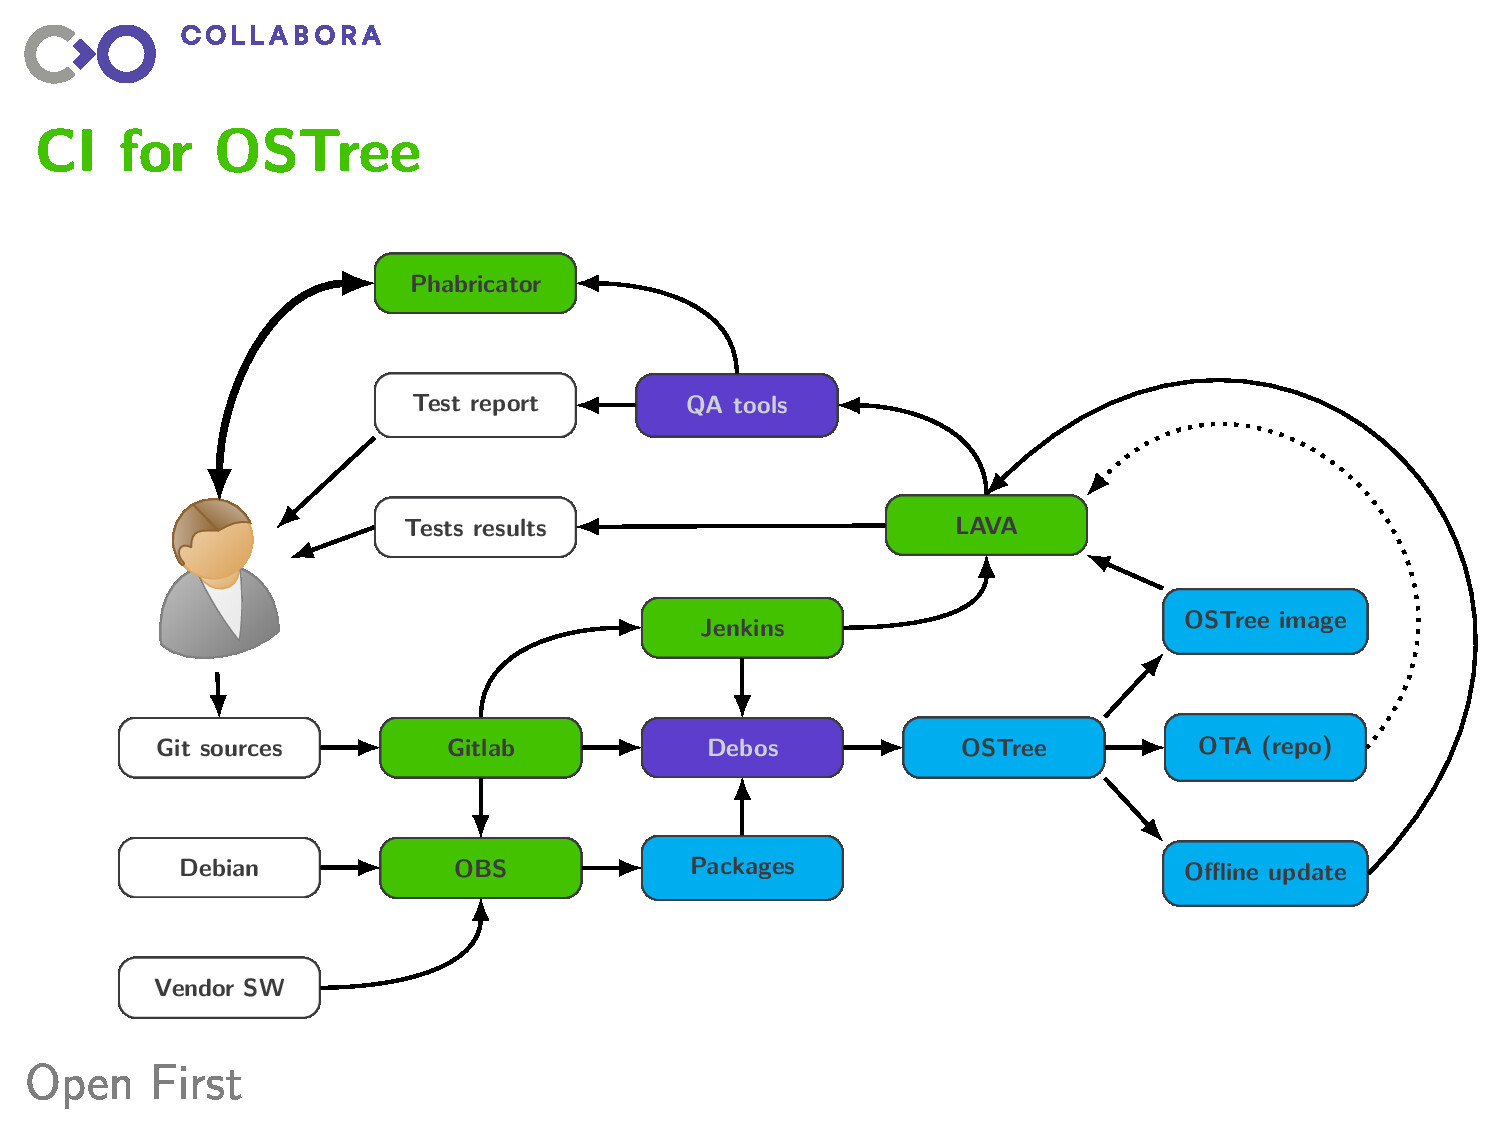
\includegraphics[width=10cm]{2019_Pynkin}  
  \label{pynkin:fig1}
\end{figure}
\end{center} 


Для обеспечения автоматической сборки и тестирования пакетов и готовых дисковых образов используются следующие системы и утилиты:

\begin{itemize}
  \item Gitlab\cite{bib10} --- хранение и ревью исходного кода;
  \item Phabricator\cite{bib11} --- управление проектом и трекер ошибок;
  \item Jenkins\cite{bib12} --- управление сборочными процессами;
  \item Open Build Service\cite{bib13} --- сборка и публикация пакетной базы;
  \item Debos\cite{bib7} --- утилита для создания загрузочных образов дисков;
  \item LAVA\cite{bib14} --- автоматическое тестирование собранных дисковых образов;
  \item QA Apertis\cite{bib15} --- тесты и набор скриптов для анализа результатов тестования, а также генерации отчетов.
\end{itemize}

В документации\cite{bib3} присутствует описание настройки ключевых компонентов для создания своей собственной инфраструктуры при необходимости.

\section*{Использованные источники}

\begin{thebibliography}{9}
\bibitem{bib1} \url{https://apertis.org}
\bibitem{bib2} \url{https://ostree.readthedocs.io}
\bibitem{bib3} \url{https://designs.apertis.org}
\bibitem{bib4} \url{https://wiki.apertis.org}
\bibitem{bib5} \url{https://gitlab.apertis.org/appfw/apertis-update-manager}
\bibitem{bib6} Пынькин Д.А., OSTree --- атомарные обновления ОС в стиле git, 2018, \url{https://lvee.org/ru/abstracts/289}
\bibitem{bib7} \url{https://github.com/go-debos/debos}
\bibitem{bib8} Пынькин Д.А., Debos --- еще одна утилита для создания ОС, 2018, \url{https://lvee.org/en/abstracts/263}
\bibitem{bib9} \url{https://github.com/go-debos/fakemachine}
\bibitem{bib9} \url{https://about.gitlab.com/}
\bibitem{bib10} \url{https://phacility.com/phabricator/}
\bibitem{bib11} \url{https://jenkins.io}
\bibitem{bib12} \url{https://openbuildservice.org/}
\bibitem{bib13} \url{https://www.lavasoftware.org/}
\bibitem{bib14} \url{https://qa.apertis.org/}
\bibitem{bib15} \url{https://gitlab.apertis.org/tests/apertis-test-cases}
\end{thebibliography}
\end{document}
